\documentclass[12pt]{report}

\usepackage[english]{babel}

\usepackage{graphicx}
\usepackage[colorlinks=true, allcolors=blue]{hyperref}

\bibliographystyle{plain}

\title{CRPL: Interim Report}
\author{Harrison Beau Barker}

\usepackage{graphicx}
\graphicspath{ {images/} }

\newcommand{\keyword}[1]{\textbf{\textit{#1}}}
\newcommand{\q}[2]{\begin{quote} #1 \cite{#2} \end{quote}}

\setlength{\parskip}{1em}
\setlength{\parindent}{0em}
\begin{document}

\maketitle
\abstract{This report is an overview of the work completed and required for the success of my project CRPL (Copyright on a public ledger). CRPL is an open-source decentralised platform aimed at removing barriers and complex legal issues from creators allowing them to create more freely without fear of copyright. 

Within this document, I will discuss the background research necessary within key areas: Blockchain, Copyright law and the current market. Technical methods and development methodologies used in the construction of this project. 	My current progress and results in smart contract development and deployment.}

\tableofcontents{}

\chapter{Keywords}

\begin{description}
  \item[Blockchain] A blockchain is essentially an immutable data structure made of hashed \keyword{blocks} not dissimilar to a linked list. Each block contains a timestamp, the actual data stored, and a hash (Ethereum uses Keccak-256 for hashing) of the previous block. this is what makes this data structure immutable and more importantly secure because once a block has been hashed you can't go back and change it otherwise the hash would be different, this also means the more blocks hashed on the chain the harder it is to change the past as new blocks depend on the validity of the previous.
  \item[Ethereum] Ethereum simply is an open-source blockchain with its own cryptocurrency Ether, however its real claim to fame is its \keyword{smart contract} functionality thanks to the Ethereum Virtual Machine (EVM) which allows for the existence of powerful concepts most importantly \keyword{state} and to be able to modify the current state. Ether is currently the second most valuable crypto currency in the world and the ethereum blockchain is the largest of its kind.
  \item[Smart Contract] As talked about previously smart contracts are pieces of software stored within the Ethereum network, these programs have an address, Ether balance, and can transact. All smart contracts are "controlled" via transaction which of course are saved to the blockchain this interaction is therefore irreversible which allows for the changing of sate and the history of state to forever be recorded.
  \item[Intellectual property] Is a blanket term describing any property created by the human intellect specifically intangible property eg; a carpenter who designs a new type of chair is only protected in terms of IP for the design or any unique building practices but not the physical chair itself which would be subject to other property laws.
  \item[Copyright] Is therefore a specific type of Intellectual property law which pertains to the copying and distribution of a work, copyright is extremely important for the protection of works as it ratifies who can essentially make money from the work.
\end{description}

\chapter{Introduction}

CRPL or \textbf{C}opy\textbf{r}ight on a \textbf{p}ublic \textbf{l}edger is an open platform for registering and managing the copyrights of a creators intellectual property secured on the publicly distributed ledger Ethereum. The immutability and public distribution of a blockchain is the essential component to the success of this platform and allows copyright registration to be placed in everyones hands.

The blockchain industry is currently booming with thousands of startups and big name players getting involved innovating with this new technology, however I believe there is a big misstep in the application of blockchain technology as generally the systems and product being made are using its as a marketing pitch not a fundamentally different way of creating a system. Most are web apps we already have but with blockchain internals whereas the application of blockchain within social and democratic issues is immense (Don and Alex Tapscott talk about this topic in more depth in their book Blockchain Revolution\cite{blockchain_revolution} which in part inspired me to develop this particular project) and should be the real focus of this new technology.

The core motivation for this project is two fold: first is the simplification or disintermediation of intellectual property rights and secondly is the decentralisation of copyright. The idea of copyright is simple however the implementation is far from, a large part of this comes from the fact that copyright existed before the internet meaning governments had to each implement their own idea of copyright this became a real problem when intellectual property went global thanks to the internet. Now each system has to sort of mesh with each others which can be extremely complex especially when it comes to smaller independent creators.

I believe my solution will solve a lot of these issues by making the protection of intellectual property easy and open.

\chapter{Background/Research}

\section{Blockchain}

The theory of a blockchain is not new \cite{origins_blockchain} but the implementation and hype around blockchains is new and extremely popular in the current day thanks to Bitcoin designed by Satoshi Nakamoto based on their white paper \cite{nakamoto2008bitcoin}. The main tenants of a blockchain are decentralisation, distribution, and immutability. Therefore for a blockchain to exist and be useful it needs people or nodes to maintain the data structure authenticate all transactions in a block and hash the current block in preparation for the next in the chain.

%TODO graphviz diagram of a blockchain?

\subsection{Technical proficiencies / limitations}

In this section I will be discussing the technical pros and cons of a blockchain system

\subsubsection{Proficiencies}

The three main selling points of blockchain technology are as follows:

\begin{enumerate}
	\item \textbf{Security} Is the core tenant of a blockchain as the cryptographic hashing strategy is what makes the data structure a chain.
	\item \textbf{Transparency} Is not intrinsic to blockchains that is down to the implementation ie: if it's public or not, however the underlying concept facilitates and promotes this open and transparent behaviour simply by the fact that nodes within a blockchain network need a copy of all transactions/previous blocks.
	\item \textbf{Decentralisation} Is definitely the most talked about benefit of blockchains and it's not a technical benefit just like transparency decentralisation is a social or philosophical debate that is made possible by the technical decisions of the blockchain architecture, mostly centred around the control and ownership of peoples data \begin{quote}"It avoids concentrations of power that could let a single person or organization take control."\cite{bohme2015bitcoin}\end{quote} 
\end{enumerate}

% blockchain in government \cite{OLNES2017355}
% trust \cite{7163223}

\subsubsection{Limitations}

Blockchain technology faces two major limitations, the largest chains in the world (Bitcoin and Ethereum) are quickly growing in size as they progress through the adoption phase of their lifecycles which has clearly pointed out scaleability problems relating to transaction speed and cost per transaction which are currently slow and expensive respectively compared to their traditional counterparts (cost experiments have borne this out in the aptly named paper "Comparing blockchain and cloud services for business process execution"\cite{rimba2017comparing} and show that business logic on a blockchain is 2 orders of magnitude more expensive than current cloud services).

Blockchains rely on \keyword{consensus protocols} which is a mathematical formula or process to determine consensus of the whole network, simply enough of the nodes/network has to agree the current state of the blockchain whenever it's modified. Currently all major chains including Bitcoin and Ethereum use a protocol called proof of work \cite{PoW} which uses the total amount of compute a node has produced as the comparable proof that can be verified by many other nodes easily. This has worked so far for these major chains however ballooning energy consumption (which can be seen in realtime at the \href{https://ccaf.io/cbeci/index}{Cambridge Bitcoin Electricity Consumption Index}), high transaction costs, and inadequate transaction processing bandwidth is forcing them to change and look for solutions.

% TODO pad this out a bit
Ethereum have decided to completely reinvent their consensus protocol with a fundamentally different protocol called proof of stake which promises reduced energy consumption, cheaper, and faster transactions \cite{PoS}

Although there have been other proposed solutions including: improving the proof of stake system by parallelising it across nodes \cite{fi12080125} or reducing the block size for a increase transaction capacity by reducing the amount of work needed per block however there will be a security trade off to balance \cite{kiayias2015speed}.

\subsection{Use of blockchain for IP protection}

I am not the first person to have thought of representing and enforcing copyright protection on a distributed blockchain, there has actually been a lot of discussion around the topic showing the clear benefits of using this technology for copyright such as transparency; \begin{quote} "Blockchain may substantially increase visibility and availability of information about copyright ownership." \cite{Copyright_in_the_blockchain_era} \end{quote} the power of smart contracts and utilising a networks cryptocurrency \begin{quote} "Smart contracts will allow automatic and instantaneous payments to designated parties, and expiration of a license after a certain amount of time." \cite{Copyright_in_the_blockchain_era} \end{quote} and simplification through the globalisation of copyright law.

Overall consensus is the addition of \keyword{smart contracts} to blockchain technology is extremely powerful particularly within copyright law to \begin{quote}"reliably automate a large volume of ‘dumb transactions’" \cite{missing_link_in_copyright_licensing}\end{quote} which will greatly help to reduce friction by removing unnecessary work and removing the expertise needed currently in the field to be properly protected.

\subsection{Use of blockchain for legal purposes}

The discussion around bringing copyright to blockchain is really apart of a larger conversation about the compatibility of any legal or even governmental workflows to be either represented or completely reinvented using blockchain technology, and it does look like that in many cases these types of problems can leverage blockchain and possibly even thrive.

First I'll look at the legal industry which is notoriously complicated requiring a great level of knowledge and expertise in the field to make sense of anything or more importantly get anything done. Logically laws make an obvious starting point for computerisation because computers are defined systems of ridged laws however this didn't make sense during the first wave of blockchains namely Bitcoin which almost entirely focused its efforts towards currency. Where as the introduction of \keyword{smart contracts} has opened up the possibilities for automated law processing massively reducing boilerplate and bulky legal work which is largely trivial but time consuming.

\begin{quote}
	"So-called ‘smart contracts’ built on blockchain technologies may prove to be the most important example yet of “self-executing, customised rules”." \cite{MILLARD2018843}
\end{quote}

Within a governmental setting blockchains \keyword{ledger} and transparency will do all the shining as essentially all governments are big collections of "things", assets, people and information. Not only are they collections but historical records and public institutions, thankfully blockchains are immutable, timestamped, secure and built for openness. Because a blockchain is just a general purpose data structure its uses are wide; \begin{quote}"keeping an overview of the authorities provided in a public organization and the ability to change the authority only if there is agreement among nodes which are classified as being higher ranked in the hierarchy." \cite{OLNES2017355}\end{quote}

\section{Copyright law}

What is the reason for "fixing" copyright? is it broken? Copyright law is old, it was first introduced from the 1700s to the 1800s with the introduction of the printing press and the first true copyright act being the Statute of Anne in 1710 which has morphed into the Copyright, Designs and Patents Act 1988 in the UK (link!!!!!!!) and the Copyright Act of 1976 in the US. The fact that each country has its own unique copyright laws (even though the international Berne Convention exists local jurisdictions still apply) exacerbated by the internet has been showing signs of cracks especially when "digital goods" are involved.

Theses issues can be broken down into three key areas: 

\begin{enumerate}
	\item \textbf{Legal transparency/complexity} Is the absolutely at the top of this list, as a creative can you be sure your work is protected in every jurisdiction possible? No you can't because the current copyrighting system is a sparse disconnected collection of closed databases. Implementing a globally open database of copyrighted works with consistent rules and digital finger printing. 
	\item \textbf{Royalty distributions (compensation)} Monetary transactions are the current forte of all major blockchains so why not simplify one of the hardest tasks for an creator, receiving payment for the use of a work of course this has become easier with the introduction of internet payments and purpose built systems like "PRS for Music" but integrating royalty payments straight into the copyright registration proves for secure and cohesive system.
	\item \textbf{Cost} Of protection a work is essentially free as the Berne Convention prohibits the registration of a work as a requirement to protection (copyright is born with the work), however legally protecting and defending authorship of a work is not free and can be devastating not to mention extremely one sided (massive record company vs band). With the help of an immutable global ledger determining who registered the work is simple. % smart contract laws??
\end{enumerate}

These problems and solutions in this section are talked about in the paper \textit{Copyright in the blockchain era: Promises and challenges} \cite{Copyright_in_the_blockchain_era}

%\section{Environment and crypto} not enough for this section

\section{The market}

%TODO probably a bit more ?
The vast majority of blockchain applications in the current day are financial for obvious reasons with the market capitalisation of cryptocurrencies being the universal metric for the blockchain markets size \cite{wood_2021}, however the health care industry has been aggressively investigating and implementing blockchain technology particularly in the secure distribution of medical data and health records \cite{8167115}, supply chain technology has seen some innovation tracking goods as they pass through a chain. 

\chapter{Methods/Technology used}

This section outlines the methods to be used in the project both technical and thinking

\section{Technical}

\begin{description}
	\item[C\#] is a a static and strongly typed object oriented programming language developed by Microsoft.
	\item[ASP.NET Core] is a web application framework built by Microsoft as an open source version to the pervious ASP.NET and can run on x86,x64 and arm architectures \href{https://docs.microsoft.com/en-us/aspnet/core/introduction-to-aspnet-core}{see}.
	\item[Angular] is an open source web application framework created by Google based on TypeScript (TypeScript is JavaScript superset built and maintained by Microsoft) used to create modern and complex web applications.
	\item[Nethereum] is a library for .NET allowing for ethereum blockchain access, interaction and smart contract deployment.
	\item[Solidity] is the language and compiler for smart contracts
%	\item[Sql vs NoSql]
	\item[Wallets] %% TODO
	\item[Nethereum code generator] When interacting with smart contacts you need information about what transactions it accepts however these two processes are going to be written in two different languages (C\# and Solidity), nethereum has a great solution that generates C\# classes for all smart contracts including transaction methods removing a cumbersome and bug prone intermediate task \href{https://docs.nethereum.com/en/latest/nethereum-code-generation/}{Nethereum code generation}.
\end{description}

\section{Methodologies}

\begin{description}
	\item[Agile] is an essential component to this projects success more specifically the application of agile principles within scrum, regular sprints and reviews is the chosen development format for this project.
	\item[TDD] is a development workflow that accepts a piece of software as successful if it passes one or more test cases usually produced before development of that piece of software, rigorous testing of software has shown immense advantages.
\end{description}

\section{Tools}

\begin{description}
	\item[Geth] is a local test chain tool which allows you to run whole pre configured development blockchains for testing before deploying to mainnet (mainnet is a common name for the production Ethereum network).
	\item[Azure DevOps] is a powerful cloud based tool which I'm using for CI (continuous integration) and CD (continuous delivery/deployment), this means whenever I commit new code to my project repo the code will be compiled, tested and deployed.
\end{description}

\chapter{Results}

\section{Smart Contracts}

A large majority of the work completed so far has been to do with smart contracts, This issue was the first and most project defining piece of work to be done as the functionality and success of the entire project is directly linked to the functionality and success of the copyright smart contracts. \href{https://github.com/MrHarrisonBarker/CRPL/commit/11c0e93bc92ad849c3cbea70db5ca637a320e5b2}{11c0e93} to \href{https://github.com/MrHarrisonBarker/CRPL/commit/2ccc3bbea3a7939e7f2012626ed91e4850a74d6f}{2ccc3bb}

Construction of a smart contract started for me with defining an interface (an interface simply is a definition of how to interact with the contract and what events the contract emits) which resulted in two interfaces separated into \href{https://github.com/MrHarrisonBarker/CRPL/blob/main/CRPL.Contracts/contracts/CopyrightBase.sol}{CopyrightBase.sol} for basic interaction with a token-esque contract and \href{https://github.com/MrHarrisonBarker/CRPL/blob/main/CRPL.Contracts/contracts/StructuredOwnership.sol}{StructuredOwnership.sol} which handles multi party ownership and consensus voting for changes to the ownership structure (based on a limited company share structure). Once the target interactions where defined it was time for the implementation of the contract this was done as an abstract contract \href{https://github.com/MrHarrisonBarker/CRPL/blob/main/CRPL.Contracts/contracts/Copyrights/Copyright.sol}{Copyright.sol} which can then be instantiated by a child for a specific type of copyright eg: \href{https://github.com/MrHarrisonBarker/CRPL/blob/main/CRPL.Contracts/contracts/Copyrights/Permissive.sol}{Permissive}.

% metadata

\section{Contract Deployment}

Once the contracts are written and compiled they then have to be "deployed" onto the \keyword{blockchain} so they can start being used. During development of the smart contracts I used \href{https://remix.ethereum.org}{Remix IDE} for compiling, deploying and transacting using their GUI but I need something programatic using .NET, the Nethereum library generates a useful API for sending deploy messages to the ethereum network so all I needed to do was connect to my local test chain and send the message. However these contracts will persist for longer than the current instance of the running software meaning I can't just keep the contract addresses in memory because if the program stops for any reason how will it know where the contracts are in the network. Therefore some persistent storage was needed in the form of a table within a MySQL database so a simple model was written to represent a \href{https://github.com/MrHarrisonBarker/CRPL/blob/main/CRPL.Data/ContractDeployment/DeployedContract.cs}{deployed contract} and using \keyword{EFCore} a database \href{https://github.com/MrHarrisonBarker/CRPL/blob/main/CRPL.Web/Migrations/20220123013118_DeployedContracts.cs}{migration} was generated and applied.

\section{Account Management}

At the time of writing this report account management and user authentication is in the early stages of development with only basic \href{https://github.com/MrHarrisonBarker/CRPL/blob/main/CRPL.Data/Account/UserAccount.cs}{UserAccount}, \href{https://github.com/MrHarrisonBarker/CRPL/blob/main/CRPL.Data/Account/UserWallet.cs}{UserWallet} and \href{https://github.com/MrHarrisonBarker/CRPL/blob/main/CRPL.Data/RegisteredWork.cs}{RegisteredWork} models written and \href{https://github.com/MrHarrisonBarker/CRPL/blob/main/CRPL.Web/Migrations/Application/20220123215316_UserAccountsAndWallets.cs}{migration} applied to the database. These models will be used to save user's information and most importantly their wallet address which will be used when registering and transferring copyrights to a user.

\chapter{Discussion}

The completion of these key project defining features (especially functional smart contracts) instills great confidence in my ability to implement all necessary functionality for a successful project outlined previously. One way of looking at this progress is a burndown chart:

\begin{figure}
	\caption{Sprint 1 burn down graph}
	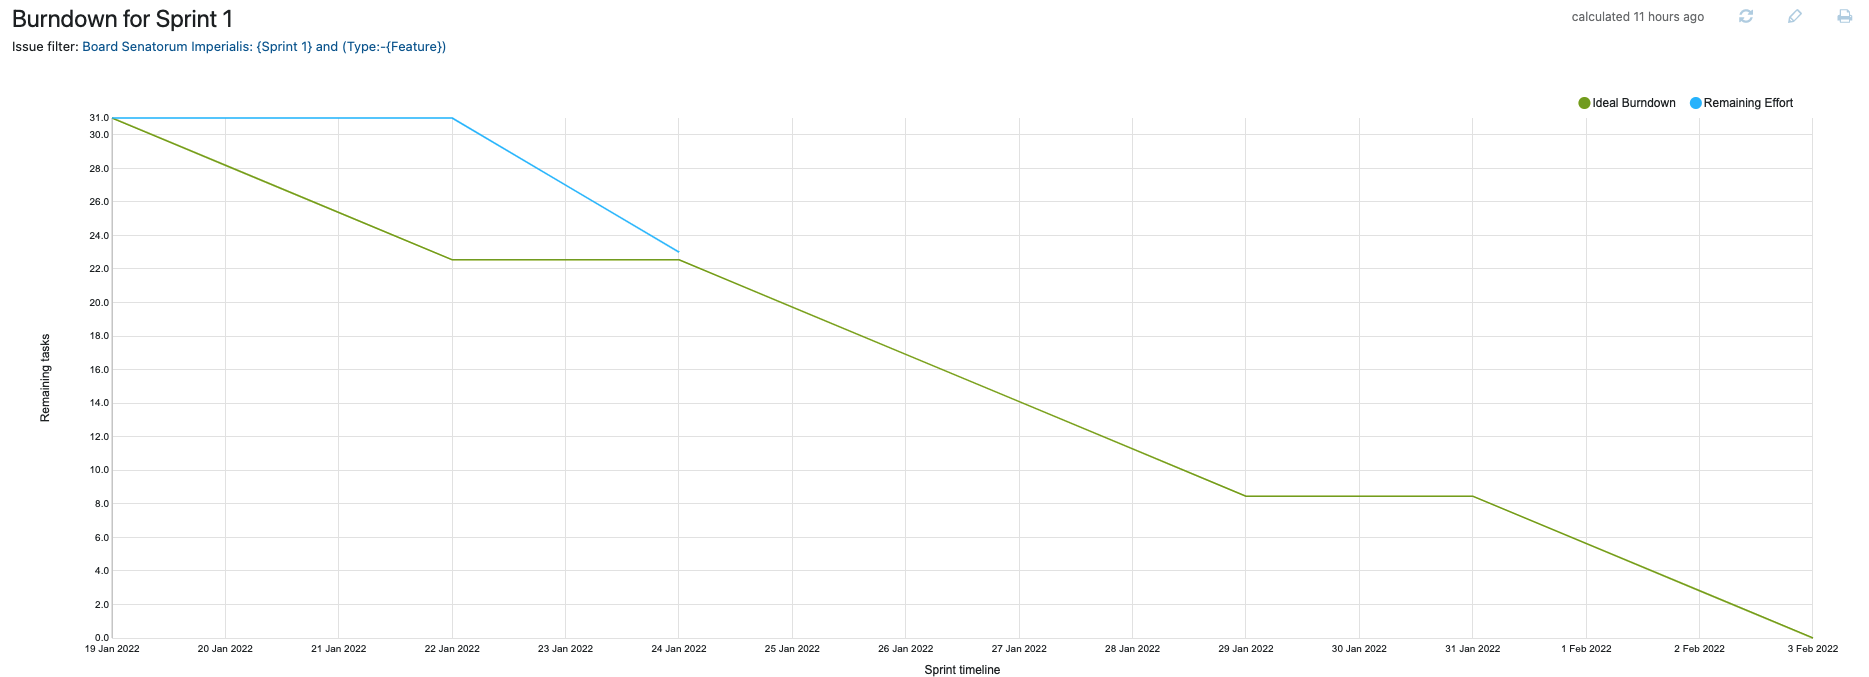
\includegraphics[width=1\textwidth]{images/sprint-1-Burn}
\end{figure}

The one problem with this graph is the perception and difference of difficulty per task, for the first four days it appears like no work is being done when in reality the first issue (CRPL-27 Copyright base interface) is the single most important issue with lots of technical and operational thinking needed, it's also the subject area I have the smallest technical knowledge.

But what we can see is that work is progressing I believe all work in this first sprint will be finished on schedule with minimal issues raised and If the succeeding sprints continue at a similar pace the project will be finished before the current deadline.


\chapter{Conclusion}

In terms of my background research it's clear blockchain technology is still in its infancy especially when is comes to practical and social solutions compared with the over saturation of financial based applications. It's also clear that copyright law itself is in need of change and that blockchain and decentralisation could be the solution it needs as this technology lends itself to implementations of law and social structures.

My results are strong and show that this project is in fact technically and physically (in terms of time) possible with the creation of a copyright smart contract with multi party ownership and consensus voting built in, this key development allows the project to function and impact global copyright practices.

\chapter{Progress and the future}

The vision and feature set of the project has not changed and all technical features are achievable within the set timeline with the current rate of progress. 

\begin{table}[h!]
\caption{Current sprint schedule}
\begin{tabular}{|l|l|l|l|}
\hline
Sprint & Start            & End              & Length  \\ \hline
1      & 19 January 2022  & 2 February 2022  & 2 weeks \\ \hline
2      & 4 February 2022  & 18 February 2022 & 2 weeks \\ \hline
3      & 20 February 2022 & 27 February 2022 & 1 week  \\ \hline
4      & 1 March 2022     & 8 March 2022     & 1 week  \\ \hline
\end{tabular}
\end{table}


\bibliography{sources.bib}

\end{document}
